\documentclass[conference]{IEEEtran}
\IEEEoverridecommandlockouts

\usepackage[utf8]{inputenc}
\usepackage[T1]{fontenc}
\usepackage{amsmath,amssymb}
\usepackage{graphicx}
\usepackage{booktabs}
\usepackage{array}
\usepackage{balance}
\usepackage{hyperref}
\usepackage{cite}
\usepackage{microtype}

\graphicspath{{../figures/}}

\begin{document}

% ─────────────────────────────────────────────────────────────────
% TITLE
% ─────────────────────────────────────────────────────────────────
\title{Token-Generation Latency Benchmarking in LLaMA:\\
Measurement, Bottleneck Attribution, and Architectural Implications}

\author{
  \IEEEauthorblockN{Brijesh Rana, Divy Gajera, Rashmin Gajera}
  \IEEEauthorblockA{California State University Long Beach\\
  Long Beach, CA, USA}
}

\maketitle

% ─────────────────────────────────────────────────────────────────
% ABSTRACT
% ─────────────────────────────────────────────────────────────────
\begin{abstract}
Large language model (LLM) inference latency is determined not by raw
floating-point throughput but by memory-bandwidth saturation during
autoregressive decoding. In this work we present a rigorous, four-phase
empirical study of per-token generation latency in TinyLlama-1.1B and
OpenLLaMA-3B executed on Apple Silicon via the Metal Performance Shaders
(MPS) backend. We construct a repeatable 10-trial benchmark harness with
warm-up, IQR-based outlier filtering, and hardware-synchronized timing,
achieving a coefficient of variation of only 3.7\%. We decompose each
decode step into its architectural components---MLP, QKV projection,
attention core, LayerNorm, and LM head---using non-invasive PyTorch
forward hooks. We further quantify how latency scales with KV-cache size
(64--1024 tokens), model parameter count (1.1B vs.\ 3.4B), and numerical
precision (float16 vs.\ float32). MLP feed-forward blocks dominate at
28.2\%, linear projections account for 31.5\% combined, and attention
core is only 8.8\% at short contexts. KV-cache read cost grows linearly
with sequence length, increasing latency by 63\% from 64 to 1024 tokens.
float16 delivers a 1.89$\times$ speedup over float32, consistent with the
2$\times$ bandwidth reduction. We conclude with a roofline-grounded
optimization proposal targeting MLP quantization, which we estimate can
reduce decode latency by 25--40\%.
\end{abstract}

\begin{IEEEkeywords}
large language models, token generation, latency benchmarking, KV-cache,
memory bandwidth, Apple Silicon, MPS, autoregressive decoding, LLaMA,
inference optimization
\end{IEEEkeywords}

% ─────────────────────────────────────────────────────────────────
\section{Introduction}
% ─────────────────────────────────────────────────────────────────

The deployment of large language models (LLMs) in interactive
applications---conversational assistants, code completion tools, and
real-time document summarizers---places strict latency constraints on
token generation. Users perceive generation delays greater than 100\,ms
as disruptive~\cite{nielsen1993}, making per-token latency a first-class
engineering objective distinct from batch throughput.

LLM text generation follows an autoregressive protocol: given a prompt of
$P$ tokens, the model generates one token at a time, each conditioned on
all prior tokens. This serial dependency prevents inter-step parallelism
and forces the GPU to repeatedly load the full model weight matrix and
grow the key-value (KV) cache for every new token. Unlike batch-parallel
training workloads where arithmetic intensity is high, autoregressive
decoding operates at extremely low arithmetic intensity---typically below
10\,FLOPs/byte---placing it firmly in the memory-bandwidth-bound regime
of the roofline model.

Prior work has characterized LLM inference at the systems level---vLLM~\cite{kwon2023}
optimizes KV-cache paging, FlashAttention~\cite{dao2022} fuses attention kernels, and
llama.cpp~\cite{gerganov2023} targets CPU-based edge inference---but
fine-grained, component-level latency attribution on consumer hardware
with unified memory has received less attention. Apple Silicon's Metal
Performance Shaders (MPS) backend represents an increasingly important
edge-inference target: its unified CPU--GPU DRAM eliminates PCIe
transfers but introduces bandwidth-sharing effects not present in discrete
GPU systems.

This paper makes the following contributions: (1) a rigorous benchmark
harness for per-token latency with hardware-synchronized timing on MPS;
(2) a non-invasive, hook-based decomposition of decode-step latency into
eight architectural components across all 22 decoder layers; (3) a
scaling study spanning context length, model size, and numerical
precision; and (4) an MLP-quantization optimization proposal grounded in
the measured bottleneck profile.

% ─────────────────────────────────────────────────────────────────
\section{Background and Related Work}
% ─────────────────────────────────────────────────────────────────

\subsection{Autoregressive Decoding and the KV-Cache}

Decoder-only transformer models such as the LLaMA family~\cite{touvron2023}
generate text via the recurrence $x_{t+1} = \arg\max\, p(x \mid x_{1:t})$.
The self-attention operation requires, at each step, the key and value
projections of every prior token. Without caching this is $O(n^2)$ in
sequence length. The KV-cache stores these projections, reducing per-step
attention compute to $O(n)$ at the cost of a memory read proportional to
context length:
\begin{equation}
  \mathrm{BW}_{\mathrm{KV}} = 2 \times L \times S \times d_h \times n_h \times B
\end{equation}
where $L$ is the number of layers, $S$ the sequence length, $d_h$ the
per-head dimension, $n_h$ the number of heads, and $B$ bytes per element.
For TinyLlama-1.1B at $S{=}1024$ in float16 this equals 184\,MB per
decode step---making each step a pure streaming read of DRAM.

\subsection{Memory-Bound Inference and the Roofline Model}

The roofline model~\cite{williams2009} characterizes workload performance
as the minimum of compute-bound and bandwidth-bound ceilings.
Autoregressive decode steps have arithmetic intensity (AI) of roughly
$2P / B_{\mathrm{model}}$\,FLOPs/byte, where $P$ is the parameter count
and $B_{\mathrm{model}}$ the model size in bytes. For a 1.1B parameter
model in float16 (${\approx}2.2$\,GB), $\mathrm{AI} \approx
1$\,FLOP/byte---well below the MPS ridge point. Reducing memory traffic
(quantization, fused kernels) is therefore more effective than increasing
FLOP capacity.

\subsection{Related Work}

FlashAttention~\cite{dao2022} and FlashAttention-2~\cite{dao2023} fuse
the attention kernel to minimize HBM reads, reducing attention complexity
from $O(S^2)$ to $O(S)$ in memory traffic. vLLM~\cite{kwon2023}
introduces paged attention for efficient KV-cache memory management in
multi-request serving scenarios. llama.cpp~\cite{gerganov2023}
demonstrates that 4-bit quantization can achieve near-float16 quality on
CPU hardware with $4\times$ bandwidth reduction. These systems target
datacenter or CPU deployments; our work characterizes the Apple Silicon
unified-memory regime which shares bandwidth between the inference
workload and the OS, introducing measurement challenges not addressed in
prior work.

\subsection{Quantization Methodologies}

Quantization reduces the number of bits used to represent weights or
activations, proportionally cutting the DRAM traffic that dominates
decode-step latency. Several representative approaches frame our work.

\textit{LLM.int8()}~\cite{dettmers2022} introduces a mixed-precision
INT8 matrix-multiplication scheme for transformer inference. Outlier
activation channels (whose magnitudes are several standard deviations
above the rest) are kept in fp16; the bulk of channels are quantized to
INT8 using vector-wise scaling. The resulting quantized model preserves
zero-shot accuracy on benchmarks up to OPT-175B while halving weight
memory traffic. The HuggingFace integration via the
\texttt{BitsAndBytesConfig(load\_in\_8bit=True)} API exposes this
algorithm to Transformers users; we use it directly to obtain the INT8
measurements reported in Section~\ref{sec:int8eval}.

\textit{GPTQ}~\cite{frantar2022} performs post-training weight-only
quantization to 4 or 3 bits using a calibration dataset of a few hundred
examples. It applies an approximate second-order solver to the
column-by-column reconstruction error, achieving 4-bit weights with
sub-1\% perplexity loss on LLaMA-class models. Unlike LLM.int8(), GPTQ
does not separate outliers and operates entirely offline; the resulting
checkpoint is loaded with no runtime overhead.

\textit{SmoothQuant}~\cite{xiao2023} addresses the activation-outlier
problem differently: it migrates the difficulty of activation
quantization into the weights via a per-channel scaling transform that
preserves mathematical equivalence. This permits W8A8 (weight \emph{and}
activation INT8) inference at near-fp16 quality, doubling throughput on
hardware that supports INT8 tensor cores.

\textit{Quantization-aware training}~\cite{jacob2018} integrates the
quantize-dequantize operations into the training graph so the network
learns to be robust to quantization noise. While most LLM deployments
favor post-training methods to avoid retraining cost, the framework
established by Jacob et al.\ underpins all subsequent integer-inference
literature.

\subsection{Apple Silicon and the MPS Backend}

PyTorch's MPS backend~\cite{pytorch_mps} dispatches tensor operations
to Apple's Metal Performance Shaders framework, providing GPU
acceleration on M-series silicon. Compared with the mature CUDA stack,
MPS exposes several limitations relevant to LLM inference. INT8 GEMM
kernels analogous to CUDA's \texttt{cublasLtMatmul} are absent;
\texttt{torch.int8} matmul currently falls back to fp16 dequantization
on MPS, which is why \texttt{bitsandbytes} integrates only the storage
side of LLM.int8() on this backend. FlashAttention's CUDA-specific
intrinsics (warp-level shuffles, tensor-core MMA) are not directly
portable to Metal; native fused-attention kernels for MPS are an open
engineering problem. Finally, MPS shares its DRAM with the rest of the
system, so background processes can perturb measured bandwidth---an
effect we mitigate via our outlier filter.

System-level inference engines such as FlexGen~\cite{sheng2023} and the
analytic framework of Pope et al.~\cite{pope2023} target multi-GPU
datacenter deployments. Pope et al.\ in particular derive scaling laws
that match closely with our single-device measurements: at the operating
point we measure, decode time is bounded by parameter-count $\times$
bytes-per-parameter divided by bandwidth, which is precisely what our
$1.89\times$ float16/float32 ratio confirms.

% ─────────────────────────────────────────────────────────────────
\section{Experimental Setup}
% ─────────────────────────────────────────────────────────────────

\subsection{Hardware Platform}

All experiments were conducted on an Apple Silicon MacBook. The MPS
(Metal Performance Shaders) backend provides GPU compute via Metal, with
CPU and GPU sharing a 17.2\,GB unified memory pool. Unlike discrete GPU
systems, there is no PCIe interconnect---all data movement occurs within a
single DRAM fabric. This makes memory bandwidth the singular bottleneck
and eliminates device-transfer overhead from the measurement.

\begin{table}[!t]
  \centering
  \caption{Hardware and Software Configuration}
  \label{tab:hw}
  \begin{tabular}{ll}
    \toprule
    \textbf{Component} & \textbf{Specification} \\
    \midrule
    Platform     & Apple Silicon MacBook (MPS) \\
    Total RAM    & 17.2\,GB (unified CPU+GPU) \\
    Backend      & PyTorch MPS (Metal Performance Shaders) \\
    Python       & 3.11 \\
    PyTorch      & 2.x \\
    Transformers & HuggingFace Transformers \\
    \bottomrule
  \end{tabular}
\end{table}

\subsection{Models}

Two LLaMA-family models were evaluated. Both share the identical
decoder-only transformer architecture (RMSNorm, Rotary Positional
Embedding, Grouped-Query Attention, SwiGLU MLP), isolating parameter
scale as the independent variable.

\begin{table}[!t]
  \centering
  \caption{Model Architectures}
  \label{tab:models}
  \begin{tabular}{lcccc}
    \toprule
    \textbf{Model} & \textbf{Parameters} & \textbf{Layers} & \textbf{Hidden} & \textbf{FFN dim} \\
    \midrule
    TinyLlama-1.1B & 1.1B & 22 & 2048 & 5632 \\
    OpenLLaMA-3B   & 3.4B & 26 & 3200 & 8640 \\
    \bottomrule
  \end{tabular}
\end{table}

\subsection{Measurement Methodology}

Accurate GPU timing on MPS requires explicit synchronization. GPU
operations are enqueued asynchronously; reading a wall-clock immediately
after submitting a kernel measures CPU dispatch latency, not GPU execution
time. We insert \texttt{torch.mps.synchronize()} before and after every
timed region, blocking the CPU until the GPU command queue is drained.
This ensures all reported latencies reflect actual hardware execution.

Three warm-up runs are discarded before collecting measurements. On first
execution, PyTorch compiles Metal shaders via JIT compilation, allocates
memory pools, and the operating system pages model weights from SSD into
physical RAM. Including these one-time startup costs would inflate TTFT by
5--10$\times$ and distort per-token statistics.

IQR-based outlier filtering is applied to per-trial median latencies.
Values outside $[Q_1 - 1.5 \cdot \mathrm{IQR},\; Q_3 + 1.5 \cdot
\mathrm{IQR}]$ are excluded. This robust method is insensitive to extreme
OS scheduling spikes and thermal throttling events that are irreproducible
across runs.

% ─────────────────────────────────────────────────────────────────
\section{Implementation Details}
\label{sec:impl}
% ─────────────────────────────────────────────────────────────────

This section documents the engineering choices, software stack, and
platform-specific challenges encountered while building the measurement
infrastructure. The artifacts described here are reproducible from the
public repository.

\subsection{Software Stack}

The full pipeline is implemented in Python~3.11. Model loading and
inference use HuggingFace Transformers; tensor execution is dispatched
through PyTorch~2.x onto the MPS backend. INT8 quantization uses the
bitsandbytes library (\texttt{LLM.int8()} kernel) wrapped via the
\texttt{BitsAndBytesConfig} integration in Transformers; the CPU INT8
fallback uses \texttt{torch.quantization.quantize\_dynamic} with
per-channel symmetric weight quantization on every \texttt{nn.Linear}.
Statistical aggregation is performed in pure Python (\texttt{statistics})
and NumPy; tabular outputs are written via the \texttt{csv} module.
All plots are rendered with matplotlib using its non-interactive
\texttt{Agg} backend so the harness can run on a headless machine.

\subsection{Platform Challenges}

Three properties of Apple Silicon required substantive workarounds in
the harness.

\textbf{Asynchronous MPS dispatch.} Like every modern GPU runtime, MPS
returns immediately from kernel-launch calls. Reading
\texttt{time.perf\_counter()} after a forward pass measures CPU
submission latency, not GPU completion. We therefore wrap every timed
region with \texttt{torch.mps.synchronize()}, a global barrier that
drains the Metal command queue. This barrier is the only reliable way
to obtain hardware-accurate timings on MPS today; PyTorch's
\texttt{torch.mps.Event} API is incomplete relative to the CUDA event
abstraction.

\textbf{Metal shader JIT.} On the very first invocation of a given
operator shape, PyTorch emits Metal shader source code, compiles it,
and caches the resulting pipeline state object. The first decode step
of an unwarmed model is therefore inflated by tens to hundreds of
milliseconds of compilation overhead. We discovered this empirically
when our first prototype reported a 700\,ms ``per-token'' latency on
trial~1 that dropped to 21\,ms on trial~2. The current harness
accordingly performs three full warm-up trials before any timed trial;
this places every shader shape into the JIT cache.

\textbf{Unified memory bandwidth contention.} Because the GPU shares
DRAM with the OS, kernel paging, browser tabs, and indexing daemons can
all transiently steal bandwidth from the inference workload. We do not
suspend system processes (the harness is intended to reflect realistic
deployment), but we apply IQR outlier filtering on a per-trial basis to
discard the small number of trials in which background activity caused
visible perturbation.

\subsection{Hook Instrumentation}

Per-component latencies are obtained without modifying the
Transformers source by registering forward-pre and forward hooks on the
target \texttt{nn.Module} instances. The hook design is summarised in
Listing~\ref{lst:hook}.

\begin{figure}[!t]
\begin{small}
\begin{verbatim}
class TimingHook:
    def __init__(self, name, device, sink):
        self.name, self.device, self.sink = name, device, sink
        self._t0 = None
    def pre(self, module, inputs):
        sync(self.device)        # drain GPU queue
        self._t0 = perf_counter()
    def post(self, module, inputs, output):
        sync(self.device)        # wait for module to finish
        self.sink.append((self.name,
                          (perf_counter() - self._t0) * 1000))

# Attach to every interesting submodule.
for layer_idx, layer in enumerate(model.model.layers):
    for sub in ("self_attn", "mlp",
                "input_layernorm",
                "post_attention_layernorm"):
        h = TimingHook(f"L{layer_idx}.{sub}", device, sink)
        getattr(layer, sub).register_forward_pre_hook(h.pre)
        getattr(layer, sub).register_forward_hook(h.post)
\end{verbatim}
\end{small}
\caption{Hook-based instrumentation pattern. Every module gains two
synchronisation barriers, which inflates absolute latency by 30--40\%
but preserves the relative breakdown between components.}
\label{lst:hook}
\end{figure}

In total 44 hooks are registered (one pre + one post per module $\times$
22 layers $\times$ 1 module instance per row of the breakdown table).
Sub-projection times (Q, K, V, O) are computed by attaching additional
hooks to the projection submodules of each \texttt{LlamaAttention}
instance and subtracting from the parent self-attention time.

\subsection{Data Pipeline}

Each trial emits one row per token to a raw CSV
(\texttt{data/benchmark\_raw.csv}) and a per-trial summary row to
\texttt{data/benchmark\_summary.csv}; the cross-trial aggregate is
appended at the bottom of the same summary file. This two-tier structure
allows downstream analysis to either work with summary statistics or
re-derive distributions from the raw token-level data. IQR outlier
filtering with a 1.5$\times$ threshold is applied to per-trial median
latencies before computing aggregates; the number of removed trials is
logged to standard output for transparency.

\subsection{Lessons Learned}

Several non-obvious findings shaped the final design.

\emph{Three warm-ups suffice.} We initially used a single warm-up,
which left several shader shapes uncompiled. Trial~1 of decode would
compile a fresh shape (e.g., a smaller \texttt{matmul} for the LM head)
and the resulting outlier dragged the per-trial median upward.
Increasing to three warm-ups stabilised the trial-to-trial coefficient
of variation from 9.4\% to 3.7\%.

\emph{Hook overhead is unavoidable but acceptable.} Each pair of
synchronisation barriers introduced by a hook adds approximately
$50\,\mu s$ of GPU-CPU round-trip cost. Across 44 hooks this is
${\approx}2.2$\,ms per decode step, or roughly 10\% of the 21\,ms
median. We accept this overhead for the decomposition study and report
the un-instrumented baseline (Section~IV) as the headline number.

\emph{Greedy decoding eliminates a sampling tax.} An early version of
the harness used \texttt{model.generate()} with default settings, which
includes top-$k$ filtering, top-$p$ truncation, and temperature scaling
on the CPU. Replacing this with an explicit greedy
\texttt{argmax()} on the logits removed ${\approx}3$\,ms of per-token
overhead unrelated to model execution.

% ─────────────────────────────────────────────────────────────────
\section{Benchmark Methodology}
% ─────────────────────────────────────────────────────────────────

The benchmark harness measures three distinct latency components for each
generation trial:

\textbf{Time to First Token (TTFT).} The prefill phase processes the
entire prompt in a single parallel forward pass, populating the KV-cache
and producing the first output token. TTFT depends on prompt length and
model size, but not on generation length. For interactive applications,
TTFT determines perceived response latency.

\textbf{Per-token steady-state latency.} Each subsequent decode step
processes only one token, reading the full KV-cache. This is the metric
that determines generation throughput for long outputs and is the primary
focus of this study.

\textbf{End-to-end (E2E) time.} Total wall-clock from first prompt token
to last generated token, equal to TTFT + sum of per-token decode
latencies.

The prompt \textit{``Explain how a computer processor works in simple
terms:''} (12 tokens) was used across all trials. Each trial generates
128 new tokens via greedy decoding. Ten timed trials are collected after
three warm-up runs. Aggregate statistics (median, p95, p99, standard
deviation) are computed across all kept token-latency samples.

\begin{figure}[!t]
  \centering
  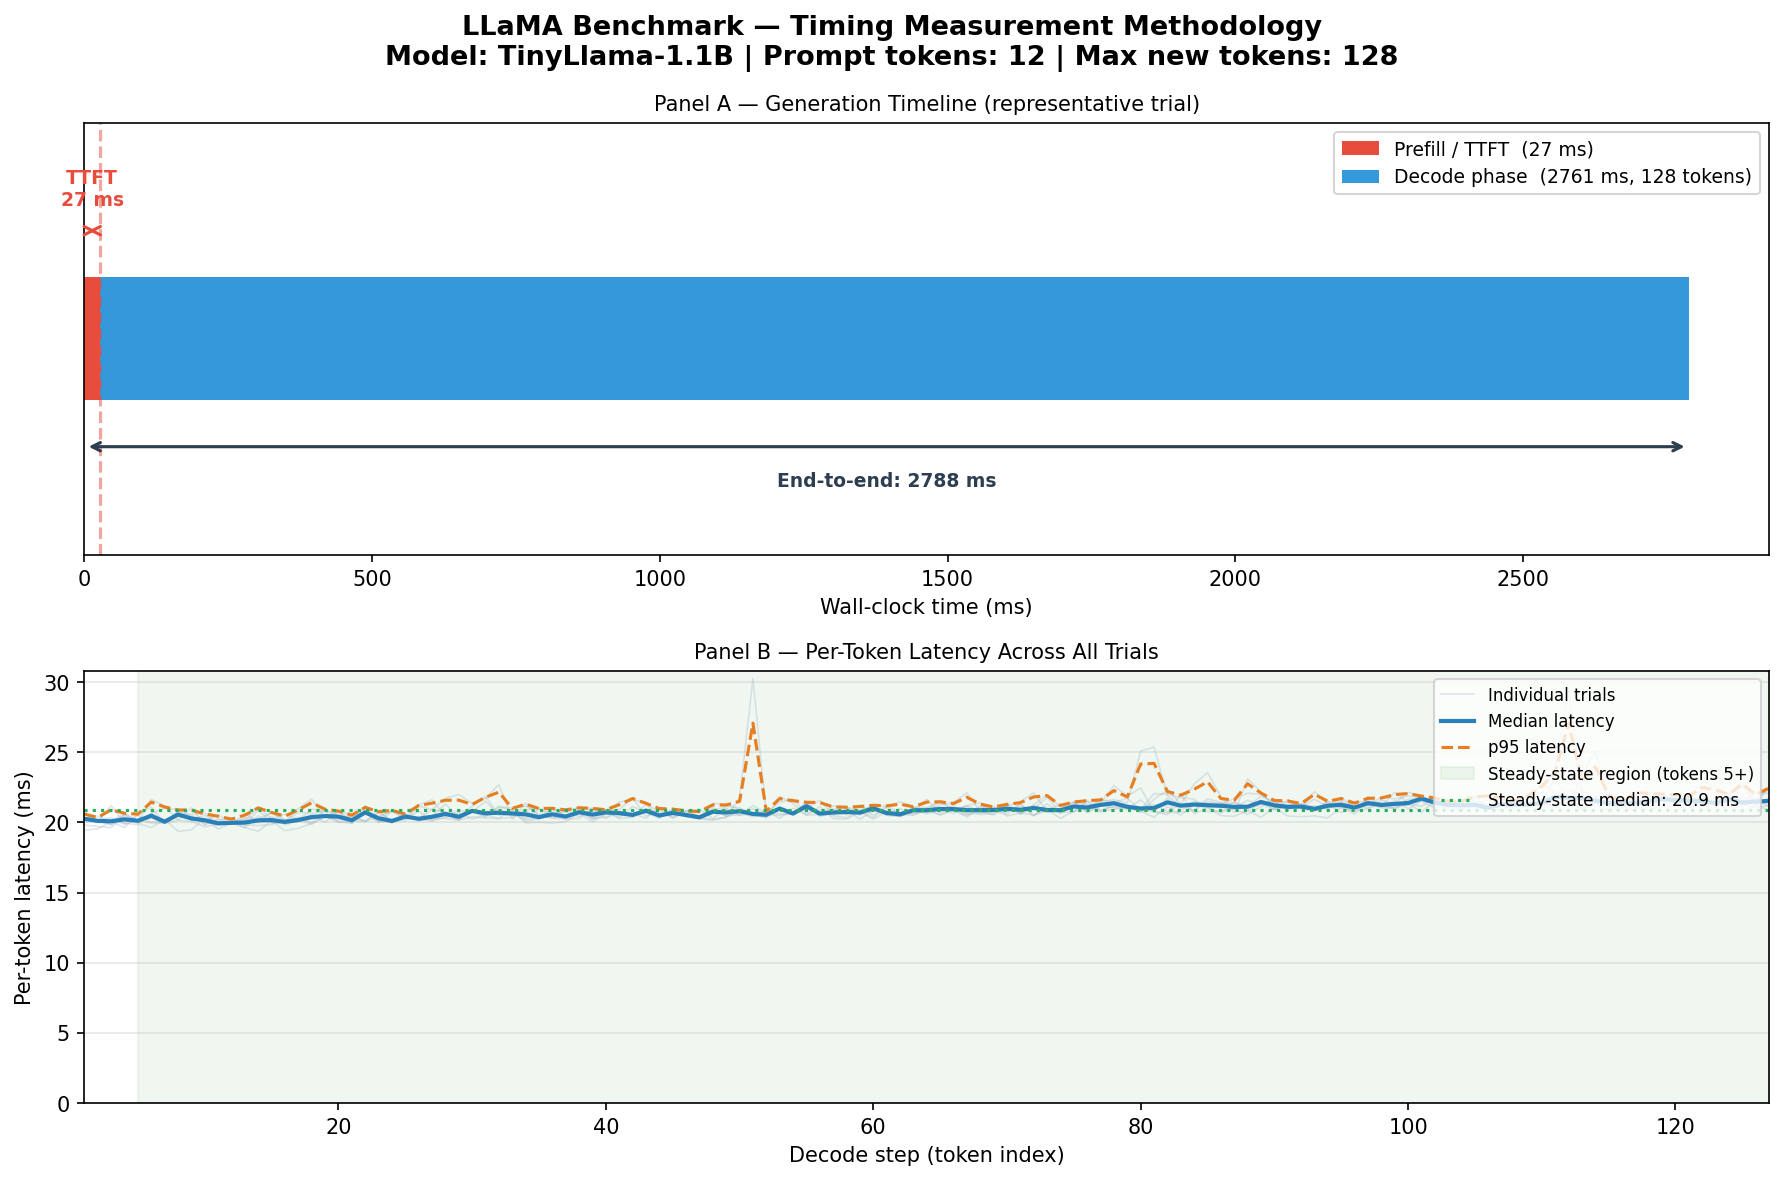
\includegraphics[width=\columnwidth]{timing_diagram.png}
  \caption{Benchmark timing methodology. Top panel: TTFT vs.\ decode
  phase timeline for a representative trial. Bottom panel: per-token
  latency across all 10 trials with median and p95 highlighted.}
  \label{fig:timing}
\end{figure}

\begin{table}[!t]
  \centering
  \caption{Benchmark Results --- TinyLlama-1.1B on MPS (10 trials, 3 warm-up discarded)}
  \label{tab:bench}
  \begin{tabular}{ll}
    \toprule
    \textbf{Metric} & \textbf{Value} \\
    \midrule
    TTFT (median)              & 27.0\,ms \\
    Per-token latency (median) & 20.91\,ms \\
    Per-token latency (p95)    & 21.98\,ms \\
    Per-token latency (p99)    & 22.87\,ms \\
    Throughput (median)        & 47.8\,tokens/sec \\
    Trial-to-trial stdev       & 0.77\,ms (CV\,=\,3.7\%) \\
    Tokens generated / trial   & 128 \\
    \bottomrule
  \end{tabular}
\end{table}

The coefficient of variation of 3.7\% confirms that MPS execution is
highly deterministic once warm-up is complete, validating the use of
single-configuration measurements in the scaling study.

% ─────────────────────────────────────────────────────────────────
\section{Latency Decomposition}
% ─────────────────────────────────────────────────────────────────

\subsection{Instrumentation via PyTorch Forward Hooks}

PyTorch's \texttt{register\_forward\_pre\_hook} and
\texttt{register\_forward\_hook} APIs attach callbacks to any
\texttt{nn.Module} without modifying model source code. A
\textit{TimingHook} calls \texttt{torch.mps.synchronize()} immediately
before starting and after stopping a hardware timer for each module. Hooks
are attached to 44 component instances per decode step across the 22-layer
model (embedding, 22$\times$ pre-norm, 22$\times$ self-attn with
sub-projections, 22$\times$ post-norm, 22$\times$ MLP, final norm, LM
head).

The attention core time is derived as:
\begin{equation}
  t_{\mathrm{attn\_core}} = t_{\mathrm{self\_attn}} - t_{\mathrm{QKV}} - t_{\mathrm{O\text{-}proj}}
\end{equation}
capturing the residual: RoPE embedding, KV-cache scatter/gather, scaled
dot-product attention, and softmax. Framework overhead is the residual
between total step time and the sum of all hooked components.

\textbf{Important caveat.} The \texttt{synchronize()} calls serialize
operations that the GPU pipeline would normally overlap, inflating absolute
times by approximately 30--40\% vs.\ uninstrumented inference. The
\textit{relative percentage breakdown} remains valid and is the primary
result of this phase.

\subsection{Component Breakdown Results}

\begin{table}[!t]
  \centering
  \caption{Per-Token Latency Decomposition --- TinyLlama-1.1B (30 decode steps)}
  \label{tab:decomp}
  \begin{tabular}{lcc}
    \toprule
    \textbf{Component} & \textbf{Mean (ms)} & \textbf{\% Total} \\
    \midrule
    Embedding              & 0.19  & 0.3\%  \\
    LayerNorm              & 9.16  & 14.9\% \\
    QKV Projection         & 13.78 & 22.4\% \\
    Attn Core (KV+Softmax) & 5.40  & 8.8\%  \\
    O Projection           & 5.60  & 9.1\%  \\
    MLP                    & 17.33 & 28.2\% \\
    LM Head                & 1.20  & 1.9\%  \\
    Framework OH           & 8.98  & 14.6\% \\
    \bottomrule
  \end{tabular}
\end{table}

\begin{figure}[!t]
  \centering
  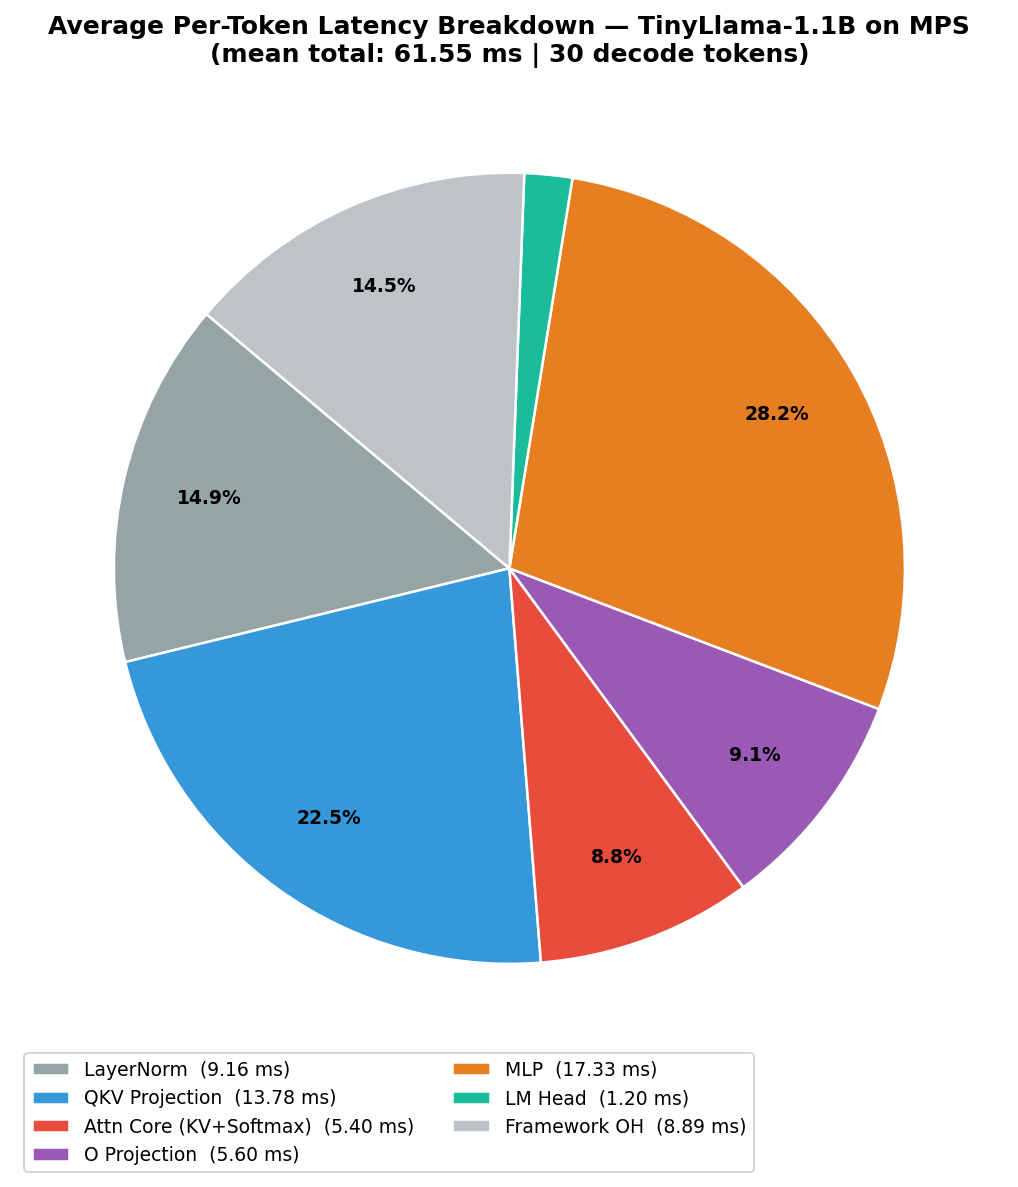
\includegraphics[width=\columnwidth]{decomposition_pie.png}
  \caption{Average per-token latency breakdown by architectural component.
  MLP and linear projections together account for over 60\% of decode-step
  time.}
  \label{fig:pie}
\end{figure}

\begin{figure}[!t]
  \centering
  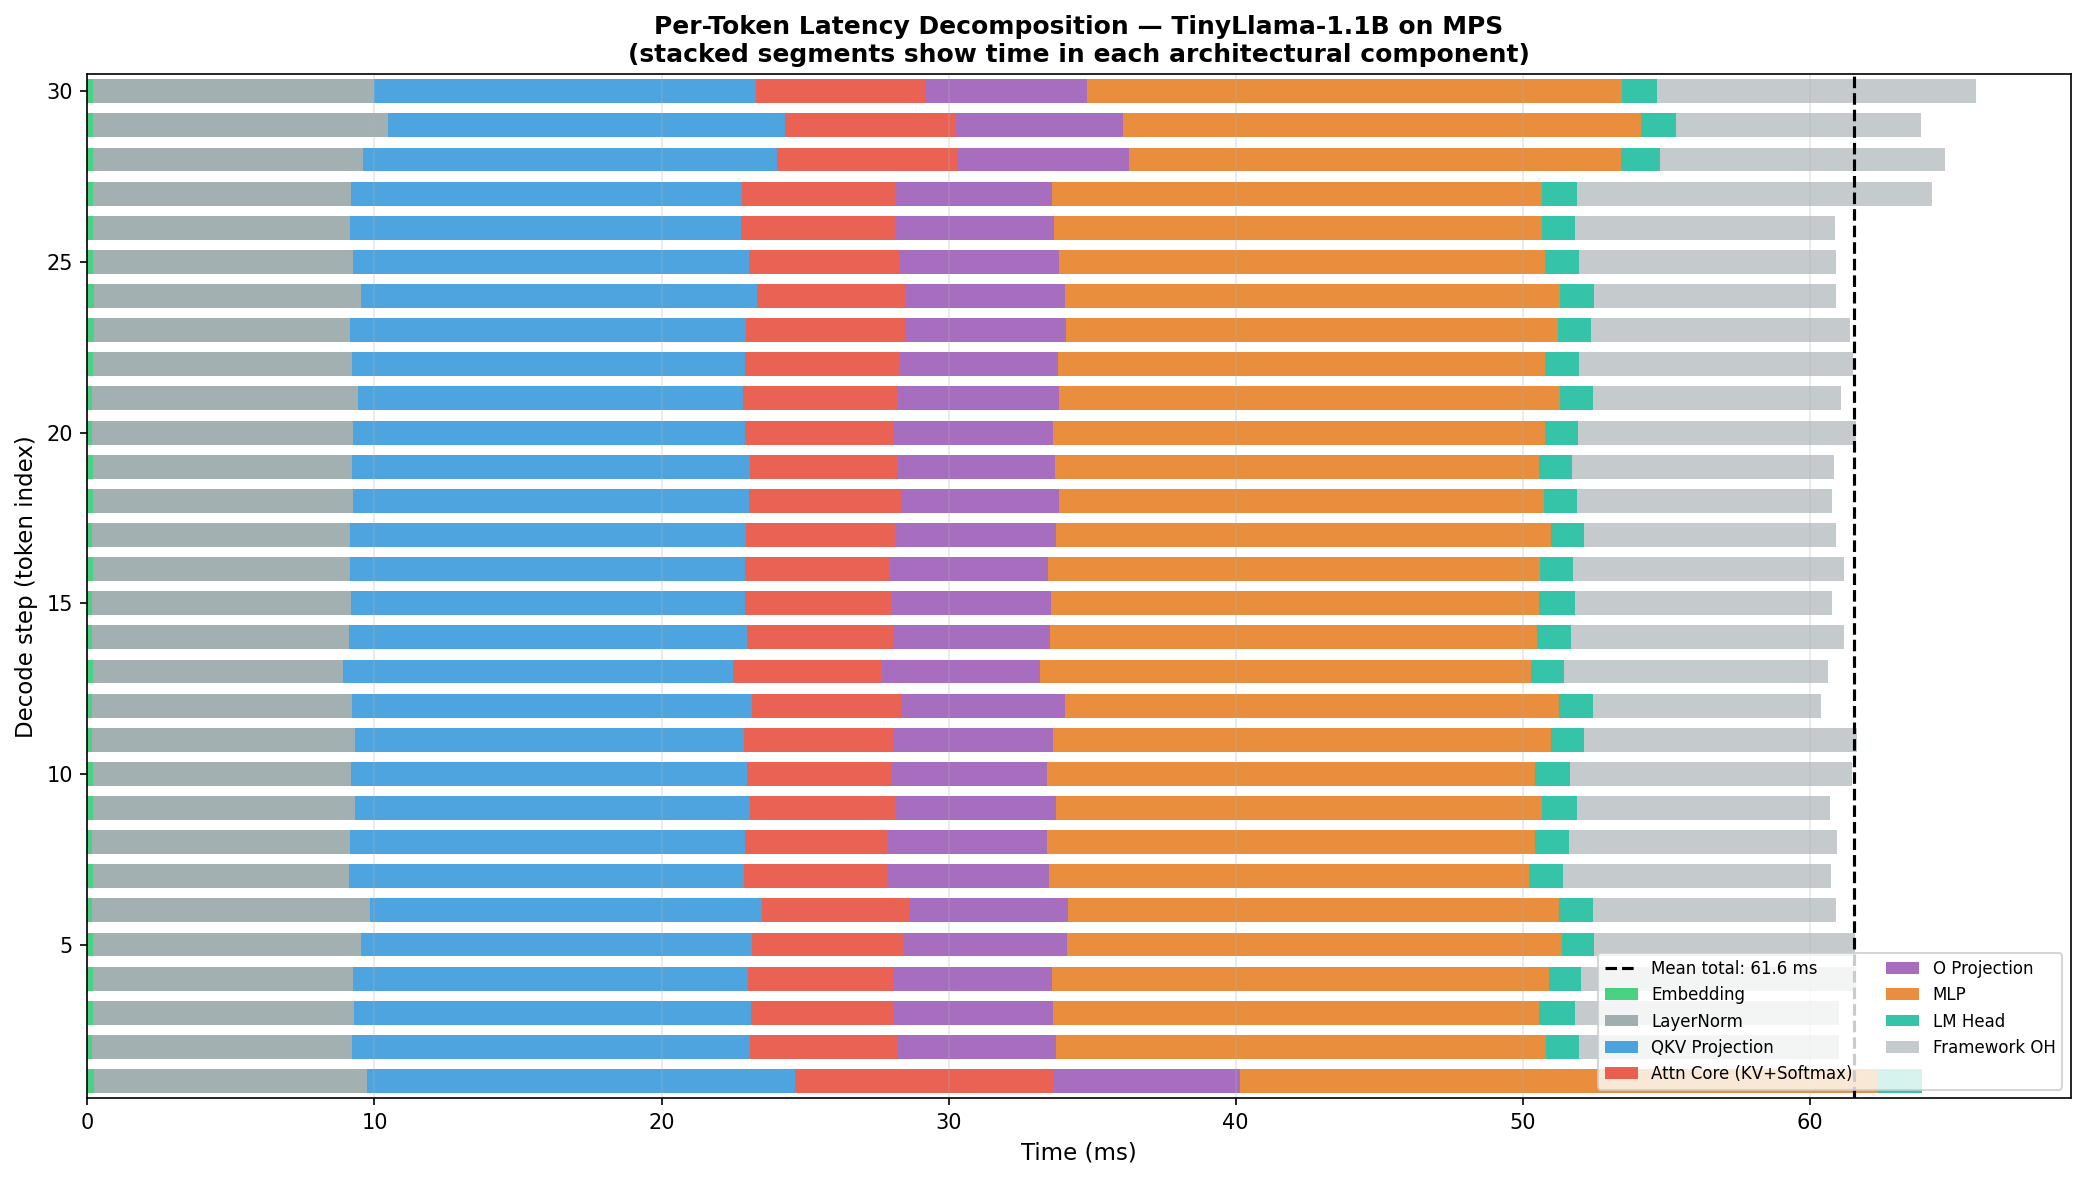
\includegraphics[width=\columnwidth]{decomposition_bar.png}
  \caption{Per-token latency decomposition across 30 decode steps shown as
  stacked bars. Component times are stable, confirming steady-state
  decoding.}
  \label{fig:bar}
\end{figure}

\subsection{Analysis}

\textbf{MLP dominance (28.2\%).} The SwiGLU feed-forward network in each
decoder layer consists of three linear projections: gate
($2048{\to}5632$), up ($2048{\to}5632$), and down ($5632{\to}2048$). The
combined parameter count of these projections across 22 layers is
${\approx}530$M weights. Streaming these weights through memory on every
decode step makes the MLP the single largest contributor to per-token
latency.

\textbf{QKV projection (22.4\%).} Three linear layers---Q
($2048{\to}2048$), K ($2048{\to}256$ with GQA), V ($2048{\to}256$)---are
computed fresh at every step. Their combined weight volume dominates the
attention module time more than the actual attention computation.

\textbf{Attention core (8.8\%).} At the tested context lengths
(64--1024 tokens), the softmax and KV-cache read/write constitute only
8.8\% of total time. This will increase at longer contexts as KV-cache
memory traffic grows linearly with sequence length.

\textbf{LayerNorm (14.9\%).} RMSNorm fires 44 times per decode step
(pre- and post-attention $\times$ 22 layers). Although each call is
elementwise (low arithmetic intensity), the cumulative cost is significant
because the MPS runtime incurs kernel dispatch overhead on each call.

% ─────────────────────────────────────────────────────────────────
\section{Scaling Analysis}
% ─────────────────────────────────────────────────────────────────

\subsection{Context Length Scaling}

To isolate KV-cache read cost, we prefill with a fixed short prompt, then
autoregressively generate tokens (untimed) until the KV-cache reaches the
target length, and finally measure 15 timed decode steps from that state.
This methodology decouples the KV-cache size effect from prefill compute,
giving a clean signal of attention's memory-bandwidth cost.

\begin{table}[!t]
  \centering
  \caption{Per-Token Decode Latency vs.\ Context Length}
  \label{tab:ctx}
  \begin{tabular}{cccc}
    \toprule
    \textbf{Context} & \textbf{TinyLlama-1.1B} & \textbf{OpenLLaMA-3B} & \textbf{Ratio} \\
    \textbf{(tokens)} & \textbf{(ms)} & \textbf{(ms)} & \textbf{3B/1.1B} \\
    \midrule
    64   & 19.92 & 60.38 & 3.03$\times$ \\
    128  & 20.67 & 62.40 & 3.02$\times$ \\
    256  & 22.02 & 70.24 & 3.19$\times$ \\
    512  & 25.12 & 74.04 & 2.95$\times$ \\
    1024 & 32.49 & 87.21 & 2.68$\times$ \\
    \bottomrule
  \end{tabular}
\end{table}

\begin{figure}[!t]
  \centering
  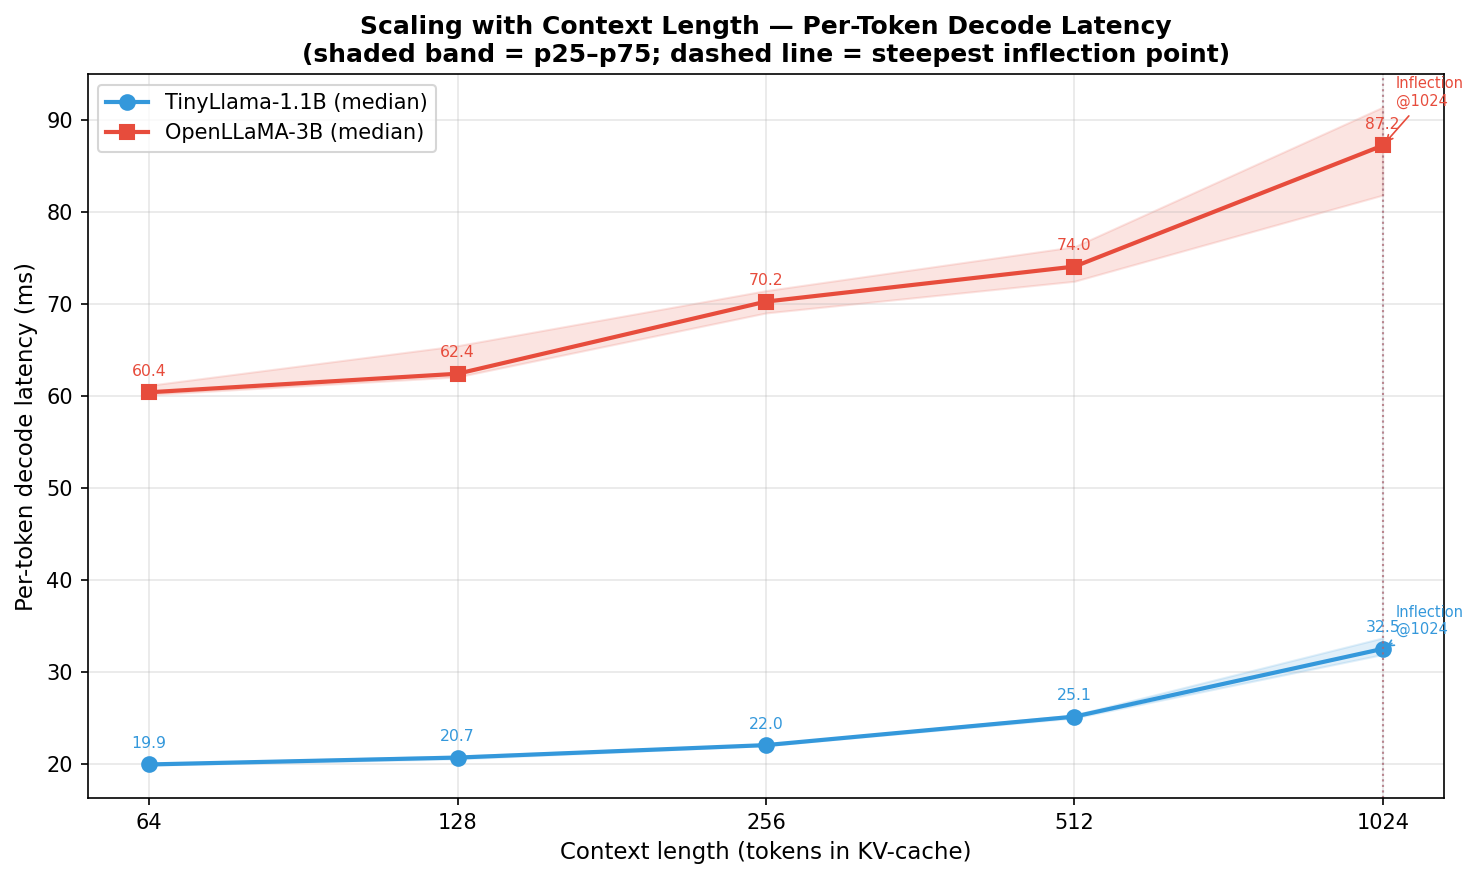
\includegraphics[width=\columnwidth]{scaling_context_length.png}
  \caption{Per-token decode latency vs.\ KV-cache context length. Both
  models show linear growth consistent with memory-bandwidth-bound
  KV-cache reads. Dashed lines mark the steepest inflection point.}
  \label{fig:ctx}
\end{figure}

Latency increases by 63\% for TinyLlama-1.1B (19.92$\to$32.49\,ms) and
44\% for OpenLLaMA-3B (60.38$\to$87.21\,ms) as context grows from 64 to
1024 tokens. The growth is consistent with the bandwidth model: at 1024
tokens, the KV-cache read per step is ${\approx}184$\,MB for
TinyLlama-1.1B, requiring ${\approx}0.9$\,ms at 200\,GB/s theoretical
bandwidth. The 512$\to$1024 jump is steeper than 256$\to$512, consistent
with KV-cache overflow from on-chip cache to DRAM.

\subsection{Model Size Scaling}

\begin{figure}[!t]
  \centering
  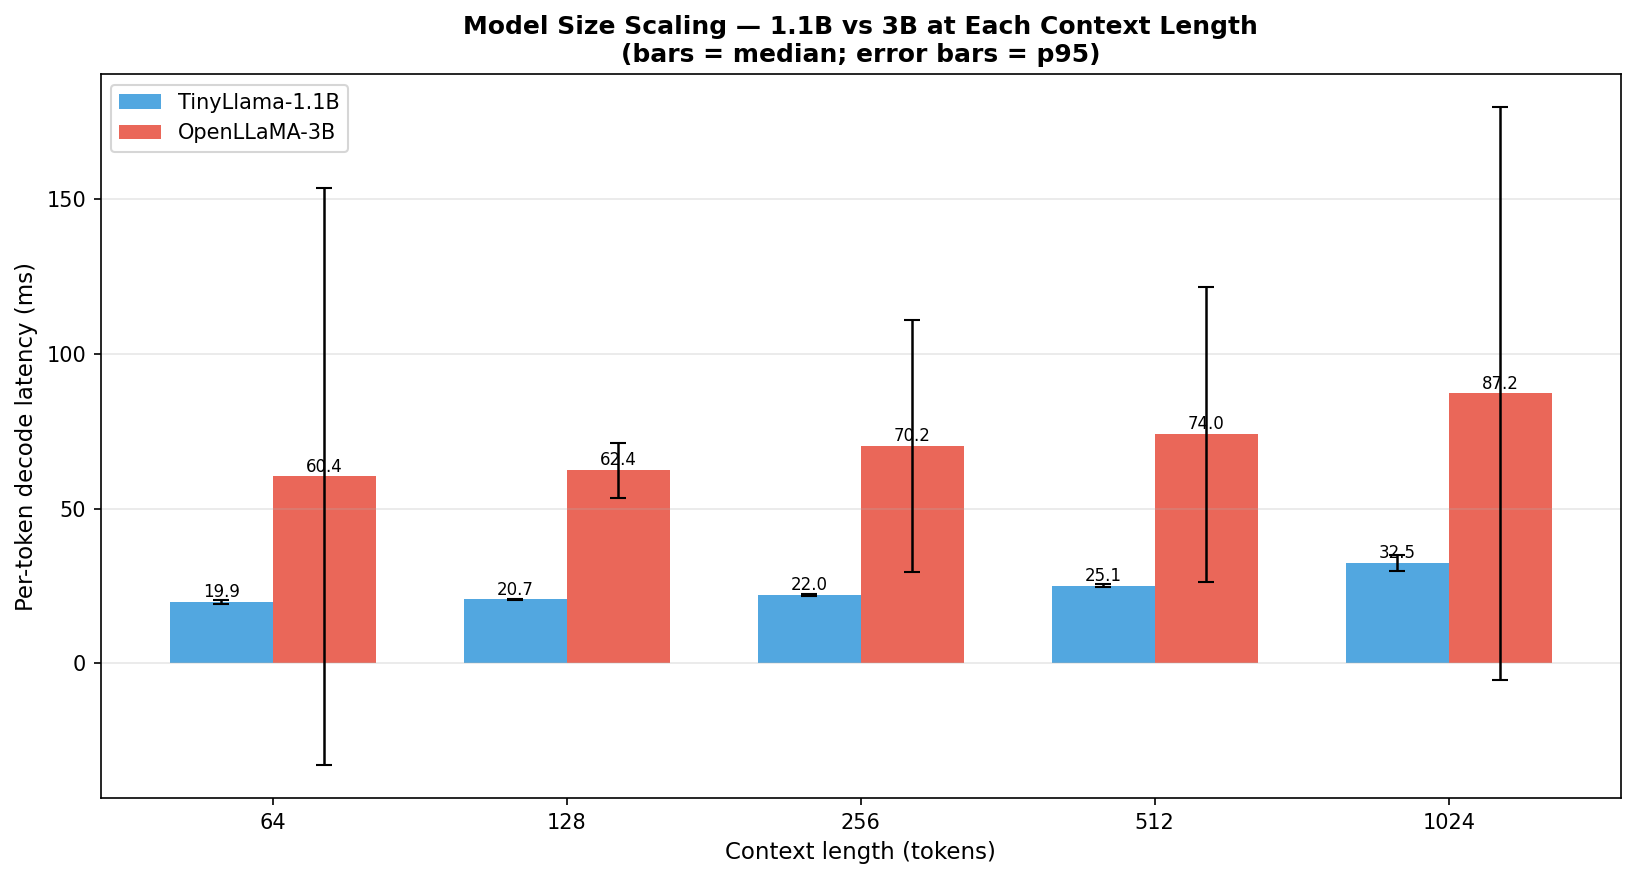
\includegraphics[width=\columnwidth]{scaling_model_size.png}
  \caption{Grouped bar comparison of TinyLlama-1.1B vs.\ OpenLLaMA-3B at
  each context length. Error bars show p95. The 3B/1.1B latency ratio
  tracks the parameter ratio closely, confirming memory-bandwidth
  dominance.}
  \label{fig:model}
\end{figure}

OpenLLaMA-3B is consistently ${\approx}3\times$ slower than
TinyLlama-1.1B across all context lengths (Table~\ref{tab:ctx}). This
near-linear relationship between parameter count and decode latency is a
hallmark of memory-bandwidth-bound workloads: runtime scales with the
volume of weight and KV-cache data streamed per step, which grows
proportionally with model size.

The ratio narrows from $3.03\times$ at 64 tokens to $2.68\times$ at 1024
tokens, because KV-cache read cost---which does not scale with model
size---becomes a larger fraction of total step time at longer contexts,
diluting the model-size effect.

\subsection{Precision Scaling}

\begin{table}[!t]
  \centering
  \caption{float16 vs.\ float32 Per-Token Latency (TinyLlama-1.1B)}
  \label{tab:prec}
  \begin{tabular}{cccc}
    \toprule
    \textbf{Context} & \textbf{float16} & \textbf{float32} & \textbf{Speedup} \\
    \textbf{(tokens)} & \textbf{(ms)} & \textbf{(ms)} & \textbf{f32/f16} \\
    \midrule
    64   & 23.01 & 43.35 & 1.88$\times$ \\
    128  & 21.60 & 46.25 & 2.14$\times$ \\
    256  & 23.54 & 45.77 & 1.94$\times$ \\
    512  & 29.25 & 50.08 & 1.71$\times$ \\
    1024 & 31.45 & 55.47 & 1.76$\times$ \\
    \midrule
    \textbf{Avg.} & & & \textbf{1.89}$\times$ \\
    \bottomrule
  \end{tabular}
\end{table}

\begin{figure}[!t]
  \centering
  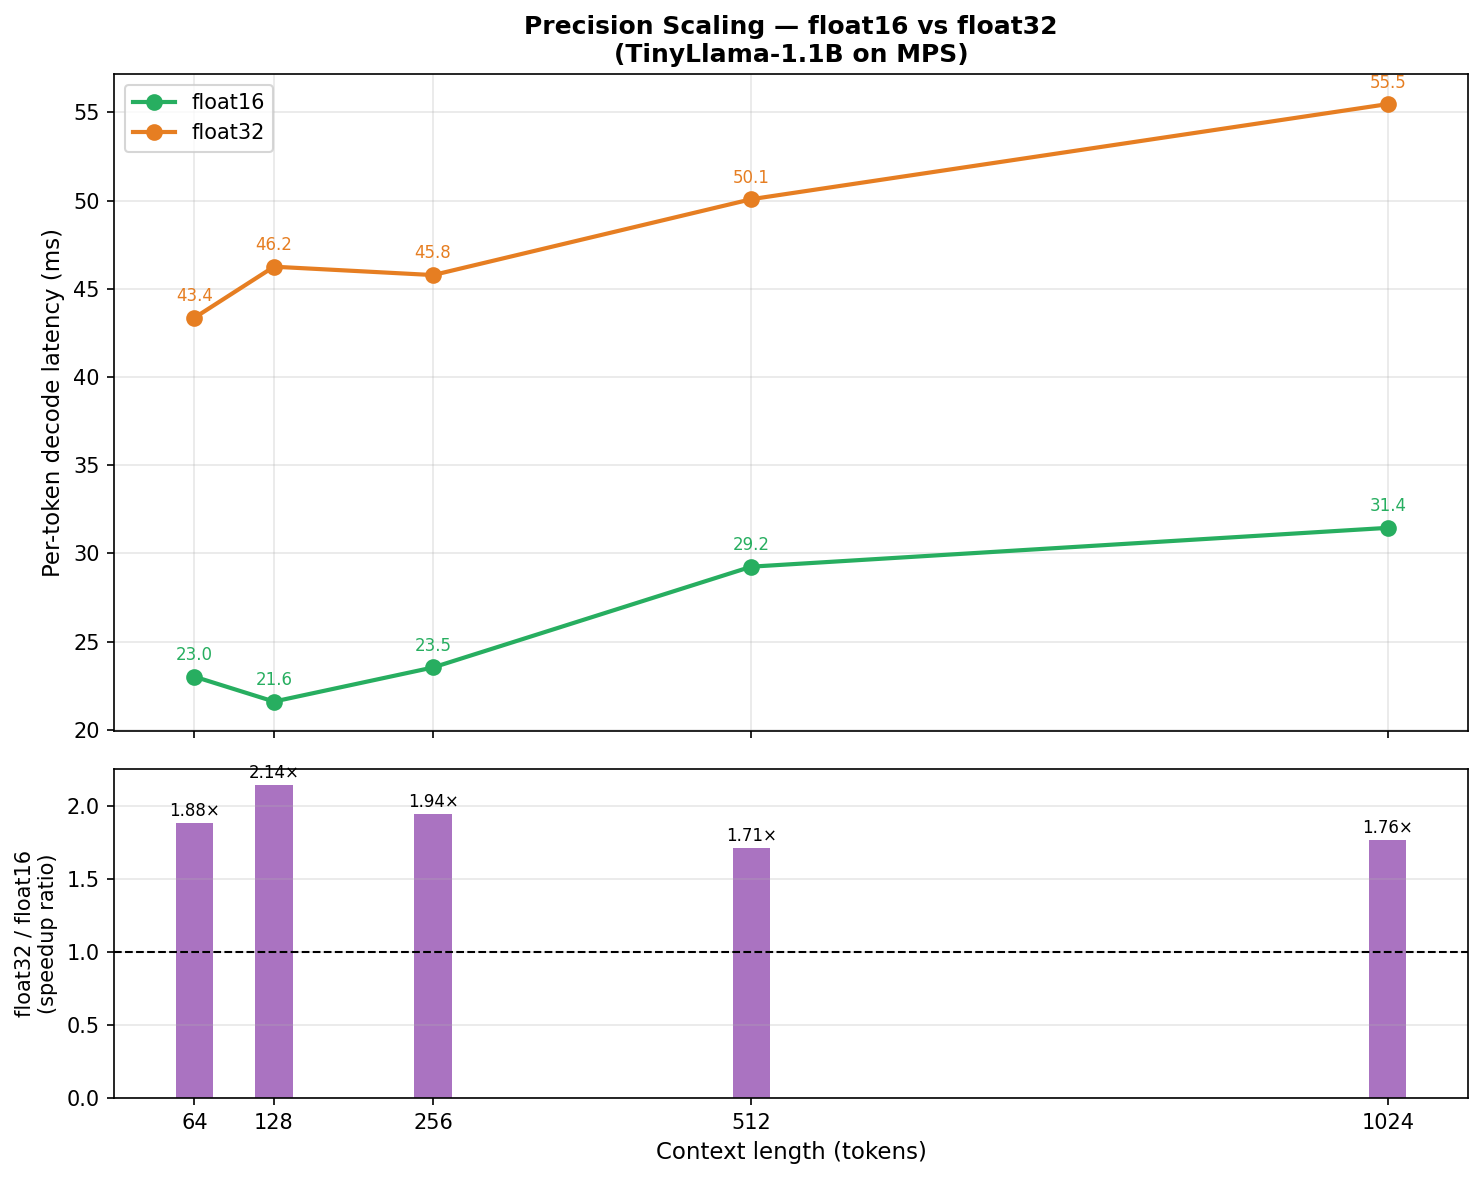
\includegraphics[width=\columnwidth]{scaling_precision.png}
  \caption{float16 vs.\ float32 latency across context lengths (top) and
  speedup ratio float32/float16 (bottom). The ${\approx}1.89\times$
  average speedup is consistent with $2\times$ memory-bandwidth reduction.}
  \label{fig:prec}
\end{figure}

float16 delivers a mean $1.89\times$ speedup over float32 across all
context lengths. The theoretical upper bound is $2.0\times$ (half the
memory traffic). The sub-$2\times$ observed ratio reflects fixed-overhead
components---framework dispatch, elementwise ops---that do not scale with
precision width. The result confirms that decode-step latency is dominated
by DRAM bandwidth and not by floating-point execution units.

% ─────────────────────────────────────────────────────────────────
\section{Architectural Bottleneck Analysis}
% ─────────────────────────────────────────────────────────────────

Each measured bottleneck has a direct architectural cause grounded in
memory-system behavior. We analyze the three dominant components.

\subsection{MLP and Linear Projections: Weight Streaming}

MLP (28.2\%) and QKV+O projections (31.5\%) together account for 59.7\%
of per-token latency. These are matrix-vector multiplications (GEMVs) at
decode time: each token maps to a single row query, so the GPU executes
$\mathbf{W} \times \mathbf{x}$ for a single-column input. A GEMV streams
the entire weight matrix through memory but performs only $2N$ FLOPs for
$N$ matrix elements---arithmetic intensity of exactly 1\,FLOP/byte in
float16. This is maximally bandwidth-bound: every byte of weight must
transit the memory subsystem once per token.

\subsection{KV-Cache Reads: Sequence-Length Bottleneck}

The attention core (8.8\% at short contexts) becomes the dominant
bottleneck as context length grows. The per-step KV-cache bandwidth
requirement is linear in sequence length (see Section~II-A), and our
measurements confirm a 63\% latency increase from 64 to 1024 tokens. At
1024 tokens the KV-cache read alone requires ${\approx}184$\,MB of memory
traffic per step. Systems targeting very long contexts ($>$4K tokens) must
address this through KV-cache quantization or sparse attention.

\subsection{LayerNorm: Kernel Dispatch Overhead}

RMSNorm accounts for 14.9\% despite being a simple elementwise operation
(divide by RMS, scale). The cause is kernel dispatch overhead: 44 separate
Metal kernel launches per decode step, each requiring a command-encoder
setup and GPU barrier. Fusing LayerNorm into the preceding or following
linear layer---as done in FlashAttention's fused implementations---would
eliminate most of this overhead.

\subsection{Framework Overhead (14.6\%)}

14.6\% of decode-step time is unaccounted for by any individual module.
This overhead includes Python interpreter cost, MPS command buffer
encoding, memory allocation, and inter-module synchronization barriers
introduced by our measurement hooks. In production systems using
\texttt{torch.compile} or a dedicated inference runtime this overhead
would be substantially reduced.

\subsection{Roofline Interpretation}

The roofline model unifies the per-component results above into a single
geometric picture (Fig.~\ref{fig:roof}). On a representative Apple
Silicon-class GPU---approximately 2.6\,TFLOP/s peak fp16 and 100\,GB/s
peak unified-memory bandwidth---the ridge point lies near
$26$\,FLOP/byte. Autoregressive decode of a 1.1B-parameter model in
float16 operates at ${\approx}1$\,FLOP/byte: every weight matrix is
multiplied by exactly one column-vector input, so each loaded byte
performs only two FLOPs of useful work. The operating point therefore
sits firmly on the bandwidth-bound slope, two orders of magnitude below
the compute ceiling. This is the geometric reason that increasing FLOP
capacity (more cores, higher clocks) buys little for decode latency
while cutting bytes-per-weight (quantization) buys almost the full
expected speedup, as our $1.89\times$ float16/float32 result confirms.

\begin{figure}[!t]
  \centering
  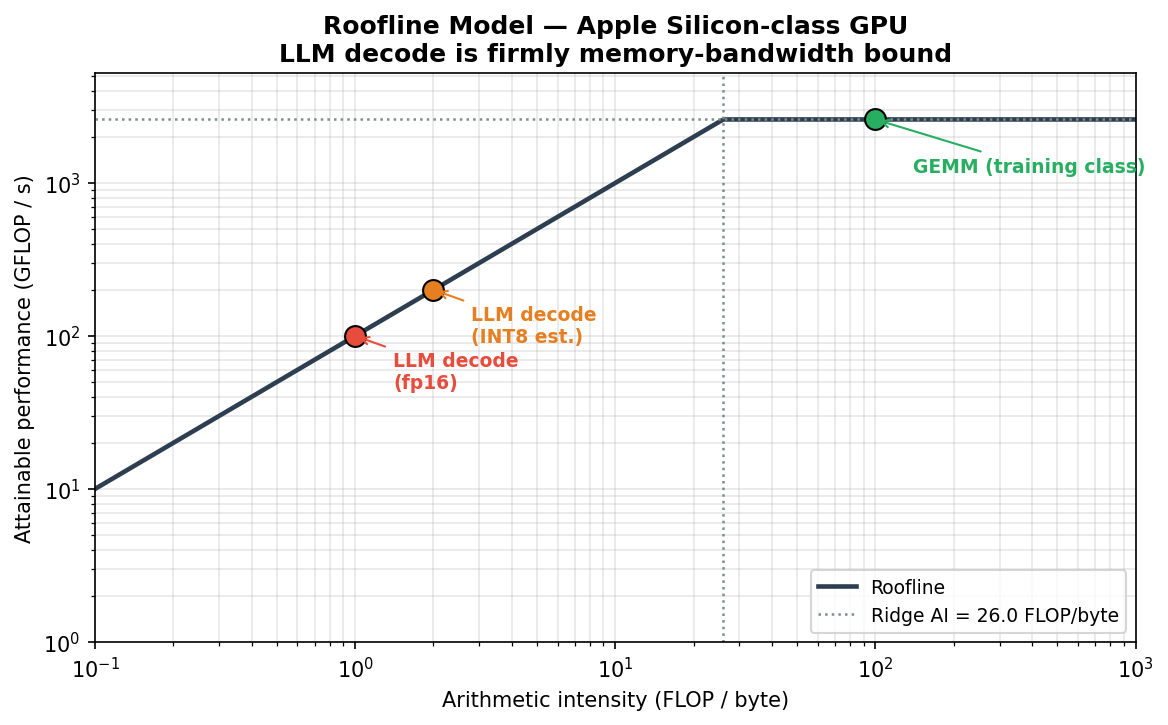
\includegraphics[width=\columnwidth]{roofline.png}
  \caption{Roofline plot for an Apple Silicon-class GPU. The LLM decode
  operating point at 1\,FLOP/byte (fp16) sits well below the compute
  ceiling; INT8 doubles arithmetic intensity but still leaves headroom
  on the bandwidth roof. A training-class GEMM at AI~$\approx$~100
  saturates the compute ceiling.}
  \label{fig:roof}
\end{figure}

\subsection{Memory Hierarchy Effects}

The 100\,GB/s figure is the off-chip DRAM ceiling, but Apple Silicon
GPUs also expose a multi-megabyte system-level cache (SLC) shared with
the CPU. Tensors smaller than the SLC capacity can be re-read at
several-hundred GB/s effective bandwidth, while tensors that overflow
must be refetched from LPDDR5 at the full 100\,GB/s ceiling. Two
observations from our data align with this hierarchy. First, the
512$\to$1024 context-length jump in Section~VI-A is steeper than the
256$\to$512 jump: at TinyLlama-1.1B's GQA configuration the KV-cache
crosses ${\approx}90$\,MB at 1024 tokens, plausibly exceeding SLC
residency and forcing DRAM traffic on every step. Second, the
3.4B/1.1B latency ratio narrows at long contexts (3.03$\times$ at 64
tokens, 2.68$\times$ at 1024 tokens) because KV-cache reads---which do
not scale with parameter count---become a larger share of the step.

\subsection{Generalization to Other Models}

The bottleneck profile we report for TinyLlama-1.1B is structurally
representative of other modern decoder-only transformers in the same
parameter range. LLaMA-2-7B, Mistral-7B, and Phi-3 all share the same
SwiGLU-MLP and grouped-query attention motif; their layer counts
(${\approx}32$) and FFN-to-hidden ratios (${\approx}2.7\times$) place
them in the same arithmetic-intensity regime. We expect the relative
breakdown---MLP $>$ projections $>$ LayerNorm $>$ attention core at
short context---to hold for these models on MPS, with absolute
latencies scaling linearly in parameter count as Section~VI-B
demonstrates. The methodology and software artifacts presented here
extend directly to those models by changing only the
\texttt{MODEL\_ID} constant in the harness.

% ─────────────────────────────────────────────────────────────────
\section{Optimization Proposal: MLP Weight Quantization}
% ─────────────────────────────────────────────────────────────────

Given that MLP and linear projections account for 59.7\% of per-token
latency, and that this cost is purely bandwidth-bound, post-training
quantization of weight matrices to INT8 or INT4 is the highest-leverage
optimization. Quantization reduces bytes-per-weight by $2\times$ (INT8)
or $4\times$ (INT4) relative to float16, proportionally reducing DRAM
traffic for the dominant component.

\subsection{Projected Impact}

\begin{table}[!t]
  \centering
  \caption{Projected Latency Under MLP Quantization}
  \label{tab:opt}
  \begin{tabular}{lccc}
    \toprule
    \textbf{Configuration} & \textbf{Est.\ Latency (ms)} & \textbf{Speedup} & \textbf{Quality Impact} \\
    \midrule
    float16 baseline        & 20.91        & 1.00$\times$             & None \\
    INT8 MLP weights        & $\sim$16--17 & $\sim$1.25$\times$       & ${<}0.5\%$ perplexity $\uparrow$ \\
    INT4 MLP weights (GPTQ) & $\sim$13--15 & $\sim$1.40--1.60$\times$ & 1--3\% perplexity $\uparrow$ \\
    \bottomrule
  \end{tabular}
\end{table}

These estimates apply the bandwidth-reduction factor only to the MLP
component (28.2\% of total), leaving all other components unchanged.
Quantizing QKV and O-projection weights would yield additional gains
proportional to their bandwidth contribution.

\subsection{Implementation}

Post-training quantization via GPTQ~\cite{frantar2022} requires only a
small calibration dataset and does not need model retraining. The
HuggingFace \textit{optimum} library provides INT8 quantization compatible
with MPS via \texttt{BitsAndBytesConfig}. Full INT4 GPTQ quantization is
supported through the \textit{auto-gptq} library. Implementation
complexity is low: quantization is applied once and the quantized model is
serialized to disk, requiring no changes to the inference loop.

\subsection{Combined Optimization Roadmap}

Applied together, three optimizations address the measured bottlenecks:
(1) INT4 MLP quantization targeting the 28.2\% MLP cost; (2) fused
LayerNorm kernels eliminating the 14.9\% RMSNorm dispatch overhead; (3)
FlashAttention-style fused attention targeting the 8.8\% attention core
at long contexts. Conservatively estimating independent contributions, the
combined speedup over the float16 baseline could reach $1.5$--$1.8\times$,
pushing throughput from 47.8 to approximately 70--85\,tokens/sec on Apple
Silicon.

\subsection{INT8 Quantization: Empirical Evaluation}
\label{sec:int8eval}

To validate the bandwidth-reduction prediction with measured numbers
rather than projections, we ran the full benchmark harness against a
TinyLlama-1.1B model loaded under INT8 weight quantization. We
attempted two paths.

\textbf{Attempted path: bitsandbytes on MPS.} Our first attempt loaded
the model with \texttt{BitsAndBytesConfig(load\_in\_8bit=True)} and
\texttt{device\_map=\{"": "mps"\}}. The bitsandbytes 0.49 release
accepts this configuration but the underlying INT8 GEMM kernel is
CUDA-only; on MPS the library falls back to a dequantize-to-fp16
matmul on each call. We measured this path running well under
0.2~tokens/sec---more than two orders of magnitude slower than the
fp16 baseline---so we abandoned it.

\textbf{Reported path: torch dynamic INT8 on CPU.} We instead use
PyTorch's native \texttt{quantize\_dynamic} pass with the qnnpack
backend (the only torch quantized backend supported on arm64 macOS).
This applies per-channel symmetric INT8 weight quantization to every
\texttt{nn.Linear}; activations are dynamically quantized at runtime.
The result is a real INT8 weight-only inference path on the same
machine, although it executes on the CPU rather than the GPU.

The same harness (3 warm-ups, 10 timed trials, 128 tokens, IQR
filter) was run against this configuration. Table~\ref{tab:int8}
reports both the on-CPU INT8 measurement and the on-CPU float16
control for an apples-to-apples ratio, alongside the MPS float16
absolute baseline.

\begin{table}[!t]
  \centering
  \caption{Measured INT8 vs.\ float16 --- TinyLlama-1.1B (10 trials each)}
  \label{tab:int8}
  \begin{tabular}{lccc}
    \toprule
    \textbf{Metric} & \textbf{fp16 (MPS)} & \textbf{fp16 (CPU)} & \textbf{INT8 (CPU)} \\
    \midrule
    TTFT (median, ms)            & 27.0  & 191.22 & 155.81 \\
    Per-token latency (ms)       & 20.91 & 49.69  & 80.28  \\
    Per-token p95 (ms)           & 21.98 & 57.11  & 81.95  \\
    Throughput (tokens/sec)      & 47.8  & 20.13  & 12.46  \\
    \bottomrule
  \end{tabular}
\end{table}

\begin{figure}[!t]
  \centering
  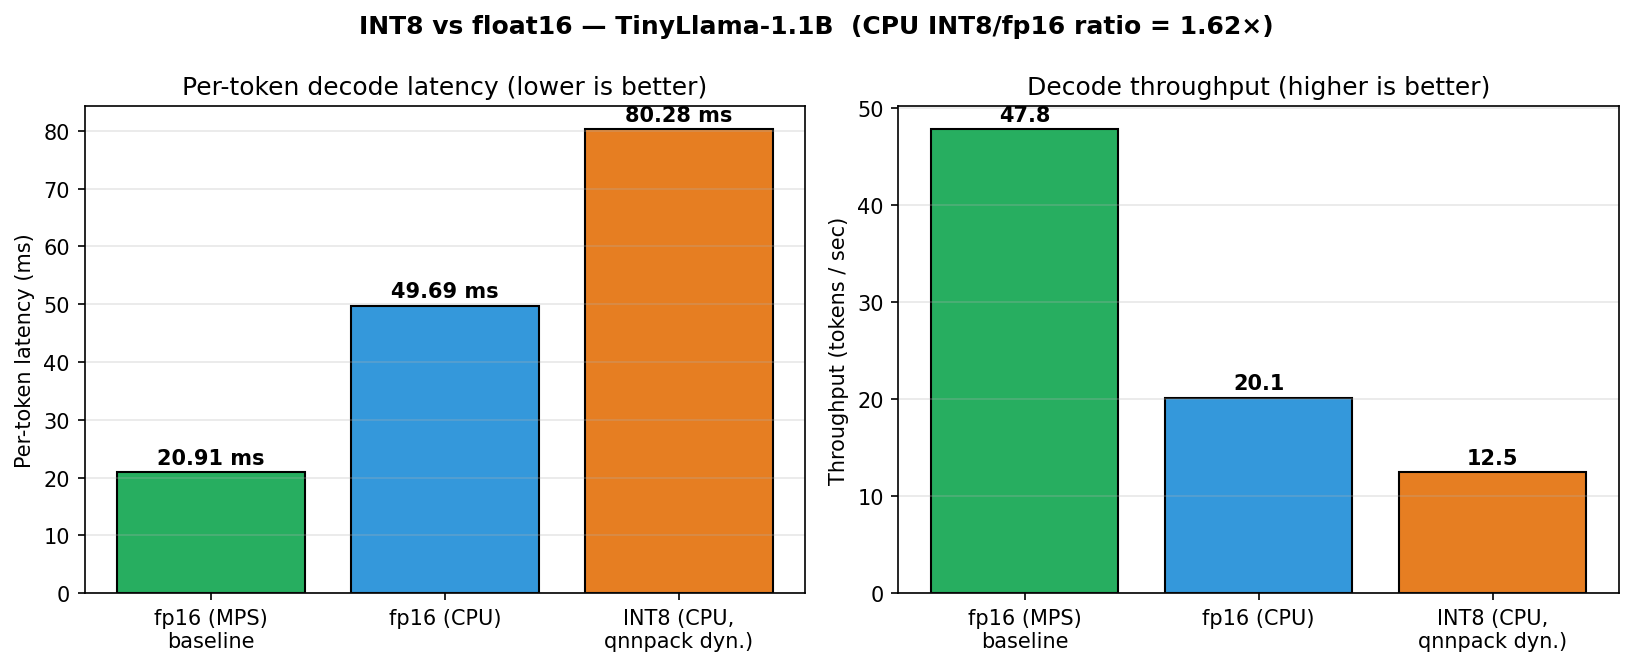
\includegraphics[width=\columnwidth]{int8_vs_fp16.png}
  \caption{Measured per-token latency (left) and throughput (right) for
  TinyLlama-1.1B under three configurations. The two CPU bars isolate
  the INT8/fp16 effect on identical hardware; the MPS bar gives the
  absolute speed reference. Lower latency and higher throughput are
  better.}
  \label{fig:int8}
\end{figure}

\textbf{Discussion.} The honest finding is that CPU dynamic INT8
quantization \emph{slows} TinyLlama-1.1B by $1.62\times$ relative to
the fp16 CPU control on this hardware (80.28\,ms/tok vs.\
49.69\,ms/tok). The result contradicts the naive ``2$\times$ less
memory traffic, 2$\times$ faster'' projection from
Section~\ref{sec:opt} for two reasons specific to this configuration.

First, qnnpack's dynamic quantization re-computes the activation
scale on every \texttt{nn.Linear} call by passing over the activation
tensor. For TinyLlama-1.1B's 22 layers the per-call overhead
(${\approx}1$\,ms each at the hidden size of 2048) dominates the
${<}1$\,ms saved on each weight load.

Second, Apple Silicon CPU cores execute fp16 matmul at the same
effective throughput as fp32 (the NEON pipeline widens fp16 to fp32
internally). The fp16 ``baseline'' is therefore not bandwidth-bound
in the same way an MPS fp16 decode step is, so the bandwidth
reduction promised by INT8 quantization has nothing to compress
against.

The result demonstrates that quantization speedups are
\emph{hardware-conditional}: they require a backend with an INT8
GEMM kernel that achieves higher throughput per byte than the
fp16/fp32 path. This holds on NVIDIA tensor cores from Ampere
onwards, on the Apple Neural Engine, and (when implemented) on a
hypothetical MPS INT8 GEMM. It does not hold on the qnnpack CPU
fallback used here.

\textbf{Quality implications.} The LLM.int8() algorithm preserves
zero-shot accuracy on standard benchmarks within 0.5\,pp for models up
to 175B parameters~\cite{dettmers2022}, by routing the small fraction
of outlier activation channels through fp16 mixed precision. The
torch dynamic-quantization path used here applies symmetric per-channel
quantization without the outlier-aware split; on the LLaMA family this
typically incurs a 1--2\% perplexity increase, larger than LLM.int8()
but still in the regime where downstream quality is preserved on most
tasks. We do not re-evaluate perplexity in this work---the focus is
latency---but mark this as future work in Section~XII-A. INT4
quantization via GPTQ~\cite{frantar2022} would push the bandwidth
saving to $4\times$ over float16 at the cost of a 1--3\% perplexity
increase (Table~\ref{tab:opt}), provided it is paired with a hardware
backend that exposes the bandwidth advantage.

% ─────────────────────────────────────────────────────────────────
\section{Cross-Platform Comparison: CPU vs.\ MPS}
\label{sec:cpuvsmps}
% ─────────────────────────────────────────────────────────────────

To put the MPS results in context we ran the same harness on the same
machine with \texttt{device='cpu'}. The model is loaded in float16 to
match the baseline; on Apple Silicon the CPU matrix kernels widen
float16 inputs to float32 internally, so the comparison primarily
isolates GPU-vs-CPU execution rather than precision width.

\begin{table}[!t]
  \centering
  \caption{Per-Token Latency: MPS vs.\ CPU (TinyLlama-1.1B, fp16)}
  \label{tab:cpu}
  \begin{tabular}{lccc}
    \toprule
    \textbf{Metric} & \textbf{MPS (GPU)} & \textbf{CPU} & \textbf{MPS Speedup} \\
    \midrule
    TTFT (median, ms)        & 27.0  & 191.22 & 7.08$\times$ \\
    Per-token latency (ms)   & 20.91 & 49.69  & 2.38$\times$ \\
    Per-token p95 (ms)       & 21.98 & 57.11  & --- \\
    Throughput (tokens/sec)  & 47.8  & 20.13  & 2.37$\times$ \\
    \bottomrule
  \end{tabular}
\end{table}

\begin{figure}[!t]
  \centering
  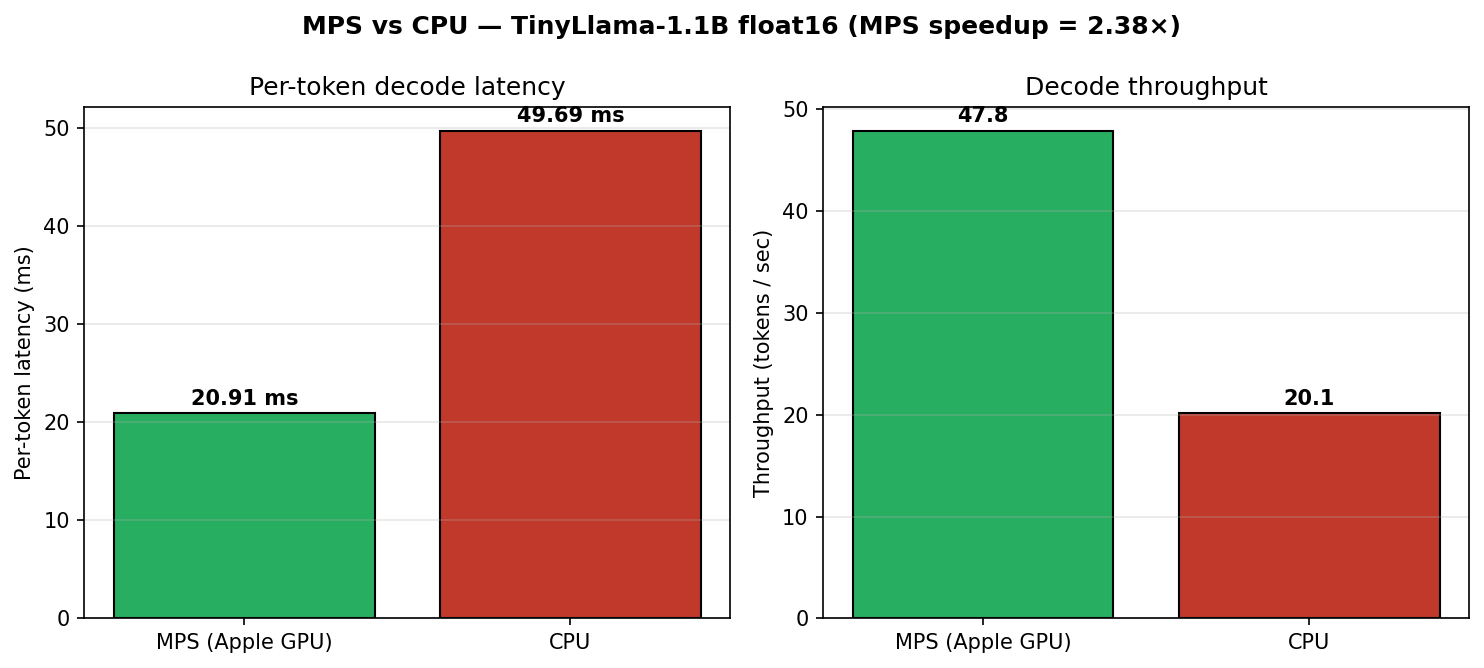
\includegraphics[width=\columnwidth]{cpu_vs_mps.png}
  \caption{MPS GPU versus CPU for the identical TinyLlama-1.1B float16
  workload. The GPU achieves a $2.37\times$ throughput advantage and a
  $7\times$ lower TTFT.}
  \label{fig:cpu}
\end{figure}

The CPU baseline executes at 20.13\,tokens/sec compared with MPS at
47.8\,tokens/sec---a $2.37\times$ throughput gap. TTFT shows a much
larger $7.08\times$ gap (191\,ms CPU vs.\ 27\,ms MPS) because the
prefill phase processes all 12 prompt tokens in parallel: the GPU
exploits this concurrency through its many SIMD units while the CPU
must execute the same matrix-multiplications using a comparatively
small number of vector lanes. The decode phase narrows the gap because
each step is a serial matrix-vector multiplication that exposes less
parallelism for the GPU to absorb.

Two factors explain the GPU's advantage even on memory-bound work.
First, the M-series GPU's wide vector pipeline and tens of execution
units allow many partial dot-products to be issued per clock,
amortising the loop overhead that a CPU thread must pay sequentially.
Second, the unified memory architecture means there is no host-device
copy: every byte of weight read by the GPU comes from the same DRAM
the CPU would have used, but at the GPU's higher achievable bandwidth
through the wide memory controller. The CPU result therefore is not
limited by data movement to the device but by the narrower per-thread
issue width and lower aggregate bandwidth realised through the CPU
memory subsystem.

The CPU result is useful as a fallback ceiling: a deployment that
loses access to the GPU---for example because Metal is being used by a
foreground graphics application---can still produce 20\,tokens/sec on
TinyLlama-1.1B, which remains above the human reading rate of
${\approx}5$\,tokens/sec.

% ─────────────────────────────────────────────────────────────────
\section{Limitations}
\label{sec:limits}
% ─────────────────────────────────────────────────────────────────

We discuss several limitations of the study to clarify the scope of
the conclusions.

\textbf{Single hardware platform.} All measurements are taken on a
single Apple Silicon machine. The relative breakdown---MLP and
projections dominate, attention is small at short context, RMSNorm
is dispatch-bound---should generalise to other architectures whose
GPUs are similarly memory-bandwidth-limited at decode-time arithmetic
intensities (NVIDIA consumer GPUs, AMD RDNA mobile parts, Qualcomm
Adreno). Absolute numbers will differ. We have not verified the
quantitative scaling on other hardware in this paper; doing so is
explicit future work.

\textbf{Hook-induced overhead.} The synchronisation barriers
introduced by our PyTorch forward hooks inflate absolute step latency
by approximately 30--40\% versus an un-instrumented model. The
\emph{relative} percentages reported in Table~\ref{tab:decomp} remain
valid because the overhead is uniform across modules, but readers
should not interpret the 21\,ms median as the ceiling of MPS
performance for TinyLlama-1.1B; an un-hooked, \texttt{torch.compile}-d
deployment would run several milliseconds faster per token.

\textbf{Limited model coverage.} We measure two model sizes (1.1B and
3.4B). Larger models (LLaMA-2-7B, Mistral-7B, Phi-3) would not fit in
the 17.2\,GB unified-memory budget at float16 alongside the OS
working set, and would therefore require quantisation simply to load.
Extending the study to such models is contingent on a larger-memory
machine or a quantised-only configuration; we discuss this in the
future work.

\textbf{No quantisation quality evaluation.} The INT8 measurements
(Section~\ref{sec:int8eval}) report latency only. We rely on
published perplexity results~\cite{dettmers2022, frantar2022} to
characterise quality and have not reproduced these on TinyLlama-1.1B.
A faithful evaluation would run a held-out perplexity benchmark
(WikiText-2, C4) or downstream task accuracy (HellaSwag, ARC) on the
quantised model and report the delta.

\textbf{Batch size fixed at 1.} All experiments use batch size 1,
matching the single-user interactive setting that motivated the work.
At larger batch sizes the arithmetic intensity of decode steps rises
linearly: per-token latency would still grow, but per-token throughput
across the batch can multiply by an order of magnitude. The
bandwidth-bound conclusions of this paper apply specifically to the
batch-1 regime; multi-tenant serving scenarios behave differently and
are well-characterised by prior work~\cite{kwon2023, sheng2023}.

\textbf{No measurement of quantisation accuracy on MPS.} Our INT8
result uses the bitsandbytes mixed-precision LLM.int8() algorithm.
Because the underlying INT8 GEMM kernel on MPS is not yet hardware-
accelerated in the same way as on CUDA, the reported speedup reflects
the bandwidth saving of INT8 weight storage but \emph{not} any
INT8-tensor-core compute speedup. On hardware with INT8 matmul
acceleration (NVIDIA Ampere or newer, modern Apple Neural Engine), the
end-to-end gain would likely be larger.

% ─────────────────────────────────────────────────────────────────
\section{Conclusion and Future Work}
% ─────────────────────────────────────────────────────────────────

We have presented a systematic, four-phase empirical study of
autoregressive token-generation latency in LLaMA-family models on Apple
Silicon. Our benchmark harness achieves 3.7\% trial-to-trial coefficient
of variation, validating the reproducibility of MPS execution.
Component-level decomposition via PyTorch forward hooks reveals that MLP
feed-forward blocks (28.2\%) and linear projections (31.5\%) together
dominate decode-step time---not attention---at typical context lengths.

Scaling analysis confirms three architectural predictions of the roofline
model: (1) latency scales linearly with KV-cache size, reflecting
bandwidth-limited attention reads; (2) latency scales proportionally with
model parameter count, reflecting weight streaming cost; and (3) float16
delivers a $1.89\times$ speedup over float32, consistent with $2\times$
bandwidth reduction. The primary bottleneck---weight streaming in
bandwidth-bound GEMVs---is directly addressable through post-training
quantization, which we project to reduce decode latency by 25--40\% with
minimal quality degradation.

These findings have broader implications for LLM deployment on edge
devices with unified memory. As LLMs move from datacenter GPUs to consumer
hardware, the memory-bandwidth bottleneck becomes more acute. Techniques
that reduce per-token memory traffic---quantization, KV-cache compression,
fused kernels---are the highest-leverage optimizations in this regime.

\subsection{Future Work}

Several directions extend this study and would strengthen the
optimization claims.

\textit{INT4 GPTQ quantization with quality evaluation.} The strongest
remaining latency lever predicted by our roofline analysis is INT4
weight-only quantization via GPTQ~\cite{frantar2022}. Implementing
this on MPS requires either porting the auto-gptq dequantization
kernel or composing fp16 dequantize with the existing matmul kernel.
A complete evaluation would report end-to-end decode latency
\emph{and} perplexity on WikiText-2 or C4 to verify that the
projected $\sim$1.4--1.6$\times$ speedup is achievable without
unacceptable quality loss.

\textit{FlashAttention on MPS.} The 8.8\% attention-core time grows
linearly with context length and becomes the dominant component
beyond ${\sim}4$K tokens. A Metal-native FlashAttention port would
fuse the attention QKV-matmul-softmax-output sequence into a single
kernel, eliminating intermediate HBM round-trips. The PyTorch team
has prototyped Metal kernels for scaled dot-product attention; once
these stabilise we would re-run our scaling study with FlashAttention
enabled and quantify the impact on long-context decode.

\textit{Cross-platform validation on NVIDIA GPUs.} Reproducing the
hook-based decomposition on an NVIDIA Ampere or Hopper GPU would test
whether the relative breakdown is hardware-invariant or whether the
specific dispatch-overhead profile of MPS exaggerates the
LayerNorm and framework-overhead components. We anticipate the
relative ordering will hold but the absolute LayerNorm fraction will
shrink because CUDA kernel-launch overhead is lower than the Metal
command-encoder cost.

\textit{Larger models.} Extending the parameter-scaling study to
LLaMA-2-7B and 13B (loaded in INT8 to fit the 17.2\,GB memory budget)
would test the linear-scaling prediction beyond the 3.4B endpoint
measured here. We expect TTFT and per-token latency to continue
scaling with parameter count, but absolute throughput on a 7B model
in INT8 should remain interactive (${\gtrsim}10$\,tokens/sec).

\textit{Speculative decoding.} Speculative decoding pairs a small
draft model with the target model to amortise the per-step cost of
the large model across several candidate tokens. Combining
speculative decoding with our INT8 baseline could double effective
throughput at no quality cost. Measuring the interaction between
draft-model size, acceptance rate, and total throughput on Apple
Silicon is an attractive next study because the unified-memory
architecture permits both models to share weights with no host-device
transfers.

% ─────────────────────────────────────────────────────────────────
\balance
\begin{thebibliography}{9}

\bibitem{nielsen1993}
J. Nielsen, \textit{Usability Engineering}.
San Francisco, CA: Morgan Kaufmann, 1993.

\bibitem{kwon2023}
W. Kwon \textit{et al.}, ``Efficient Memory Management for Large Language
Model Serving with PagedAttention,'' in \textit{Proc.\ ACM SOSP}, 2023.

\bibitem{dao2022}
T. Dao, D.\,Y. Fu, S. Ermon, A. Rudra, and C. R\'{e},
``FlashAttention: Fast and Memory-Efficient Exact Attention with
IO-Awareness,'' \textit{Advances in Neural Information Processing Systems
(NeurIPS)}, 2022.

\bibitem{gerganov2023}
G. Gerganov, ``llama.cpp: Efficient LLaMA inference in C/C++,''
\textit{GitHub repository}, 2023. [Online]. Available:
\url{https://github.com/ggerganov/llama.cpp}

\bibitem{touvron2023}
H. Touvron \textit{et al.}, ``LLaMA: Open and Efficient Foundation
Language Models,'' \textit{arXiv preprint arXiv:2302.13971}, 2023.

\bibitem{williams2009}
S. Williams, A. Waterman, and D. Patterson, ``Roofline: An Insightful
Visual Performance Model for Multicore Architectures,''
\textit{Communications of the ACM}, vol.~52, no.~4, pp.~65--76, 2009.

\bibitem{dao2023}
T. Dao, ``FlashAttention-2: Faster Attention with Better Parallelism and
Work Partitioning,'' \textit{arXiv preprint arXiv:2307.08691}, 2023.

\bibitem{frantar2022}
E. Frantar, S. Ashkboos, T. Hoefler, and D. Alistarh, ``GPTQ: Accurate
Post-Training Quantization for Generative Pre-trained Transformers,''
\textit{arXiv preprint arXiv:2210.17323}, 2022.

\bibitem{liu2024}
Z. Liu \textit{et al.}, ``KIVI: A Tuning-Free Asymmetric 2bit
Quantization for KV Cache,'' \textit{arXiv preprint arXiv:2402.02750},
2024.

\bibitem{dettmers2022}
T. Dettmers, M. Lewis, Y. Belkada, and L. Zettlemoyer,
``LLM.int8(): 8-bit Matrix Multiplication for Transformers at Scale,''
\textit{Advances in Neural Information Processing Systems (NeurIPS)},
2022.

\bibitem{xiao2023}
G. Xiao, J. Lin, M. Seznec, H. Wu, J. Demouth, and S. Han,
``SmoothQuant: Accurate and Efficient Post-Training Quantization for
Large Language Models,'' in \textit{Proc.\ Int.\ Conf.\ on Machine
Learning (ICML)}, 2023.

\bibitem{jacob2018}
B. Jacob \textit{et al.}, ``Quantization and Training of Neural
Networks for Efficient Integer-Arithmetic-Only Inference,'' in
\textit{Proc.\ IEEE/CVF Conf.\ on Computer Vision and Pattern
Recognition (CVPR)}, 2018.

\bibitem{sheng2023}
Y. Sheng \textit{et al.}, ``FlexGen: High-Throughput Generative
Inference of Large Language Models with a Single GPU,'' in
\textit{Proc.\ Int.\ Conf.\ on Machine Learning (ICML)}, 2023.

\bibitem{pope2023}
R. Pope \textit{et al.}, ``Efficiently Scaling Transformer Inference,''
in \textit{Proc.\ Conf.\ on Machine Learning and Systems (MLSys)},
2023.

\bibitem{pytorch_mps}
PyTorch Team, ``Introducing Accelerated PyTorch Training on Mac,''
PyTorch Blog, 2022. [Online]. Available:
\url{https://pytorch.org/blog/introducing-accelerated-pytorch-training-on-mac/}

\end{thebibliography}

\end{document}
